\appendix

\onecolumn
\section{Algorithmic Typing Rules}
\label{sec:algo-type-check}

\begin{figure*}[h]
\centering
\judgbox{\Delta_{in} ; \Gamma |- e : A ; \Delta_{out}}{~~Under input contexts $\Delta_{in}$ and
  $\Gamma$, expression~$e$ has intuitionistic type $A$ and output context $\Delta_{out}$.}
\begin{mathpar}
\Infer{a-var}
{\Gamma(x) = A}
{\Delta; \Gamma |- x : \Delta; \Gamma; A}
%
\and
%
\Infer{a-unit}
{ }
{\Delta ; \Gamma |- \eUnit : \Delta; \Gamma; \tyUnit}
%
\and
%
\Infer{a-pair}
{\Delta_1; \Gamma |- e_1 : \Delta_2; \Gamma; A_1\\\\
\Delta_2; \Gamma |- e_2 : \Delta_3; \Gamma; A_2}
{\Delta_1; \Gamma |- \ePair{e_1}{e_2} : \Delta_3; \Gamma;  \tyProd{A_1}{A_2}}
%
\and
%
\Infer{a-inj}
{i \in \{1, 2\}\\\\
\Delta_1; \Gamma |- e : \Delta_2; \Gamma; A_i}
{\Delta_1 ; \Gamma |- \eInj{i}{e} : \Delta_2; \Gamma; \tySum{A_1}{A_2}}
%
\and
%
\Infer{a-ref}
{\Delta_1; \Gamma |- e : \Delta_2; \Gamma; A}
{\Delta_1; \Gamma |- \eRef{e} : \Delta_2; \Gamma; \tyRef{A}}
%
\and
%
\Infer{a-split}
{\Delta_1; \Gamma |- e_1 : \Delta_2; \Gamma; \tyProd{A_1}{A_2}\\\\
\Delta_2; \Gamma,x_1:A_1, x_2: A_2 |- e : \Delta_3; \Gamma; B}
{\Delta_1; \Gamma |- \eSplit{e_1}{x_1}{x_2}{e_2} : \Delta_3; \Gamma; B}
%
\and
%  
\Infer{a-case}
{\Delta_1; \Gamma |- e : \Delta_2; \Gamma; \tySum{A_1}{A_2}\\\\
\Delta_2; \Gamma,x_1:A_1 |- e_1 : \Delta_3; \Gamma; B\\\\
\Delta_2; \Gamma,x_2:A_2 |- e_2 : \Delta_3; \Gamma; B}
{\Delta_1; \Gamma |- \eCase{e}{x_1}{e_1}{x_2}{e_2} : \Delta_3; \Gamma; B}
%
\and
%
\Infer{a-get}
{\Delta_1, \wrtok; \Gamma |- e : \tyRef{A} ; \Delta_2}
{\Delta_1, \wrtok; \Gamma |- \eGet{e} : A ; \Delta_2}
%
\and
%
\Infer{a-set}
{\Delta_1, \wrtok; \Gamma |- e_1 : \tyRef{A} ; \Delta_2\\\\
\Delta_2; \Gamma |- e_2 : A ; \Delta_3}
{\Delta_1, \wrtok; \Gamma |- \eSet{e_1}{e_2} : \tyUnit ; \Delta_3}
%
\and
%
\Infer{a-fix}
{\emptyctxt; \Gamma,x : \tyArr{A}{\footnotesize m}{A} |- e : \emptyctxt; \Gamma; \tyArr{A}{\footnotesize m}{A}}
{\Delta; \Gamma |- \eFix{x}{e} : \Delta; \Gamma; \tyArr{A}{\footnotesize m}{A}}
%
\and
%
\Infer{a-let}
{\Delta_1; \Gamma |- e_1 : \Delta_2; \Gamma; A\\\\
\Delta_2; \Gamma, x:A |- e_2 : \Delta_3; \Gamma; B}
{\Delta_1; \Gamma |- \eLet{x}{e_1}{e_2} : \Delta_3; \Gamma; B}
%
\and
%
\Infer{a-let!}
{\Delta_1; \Gamma |- e_1 : \Delta_2; \Gamma; A\\\\
\Delta_2; \Gamma, x:A |- e_2 : \Delta_3; \Gamma; B}
{\Delta_1; \Gamma |- \eLetBang{x}{e_1}{e_2} : \Delta_3; \Gamma; B}
%
\and
%
\Infer{a-abs}
{\emptyctxt ; \Gamma, x:A |- e : \emptyctxt; \Gamma; B}
{\Delta ; \Gamma |- \eLam{x}{e} : \Delta; \Gamma; \tyArr{A}{\footnotesize m}{B}}
%
\and
%
\Infer{a-app}
{\Delta_1; \Gamma |- e_2 : \Delta_2; \Gamma; A\\\\
\Delta_2; \Gamma |- e_1 : \Delta_3; \Gamma; \tyArr{A}{\footnotesize m}{B}}
{\Delta_1; \Gamma |- \eApp{e_1}{e_2} : \Delta_3; \Gamma; B}
%
\and
%
\Infer{a-nu}
{\Delta_1, x_1: \tyRd{S} ; \Gamma, x_2 : \tyWr{S} |- e : A ; \Delta_2}
{\Delta_1; \Gamma |- \eNu{(x_1, x_2)}{e} : A; \Delta_2}
%
\and
%
\Infer{a-wr}
{\emptyctxt; {\Gamma}_S |- e_1 : S ; \emptyctxt\\
\Delta_1; \Gamma |- e_2 : \tyWr{S} ; \Delta_2}
{\Delta_1, \wrtok; \Gamma|- \eWr{e_1}{e_2} : \tyUnit; \Delta_2}
%
\and
%
\Infer{a-letrd}
{\Delta_1; \Gamma |- e_1 : \tyRd{S}; \Delta_2\\\\
\Delta_2, \wrtok, x_1 : \tyBang{S}, x_2 : \tyRd{S} ; \Gamma |- e_2 : A ; \Delta_3}
{\Delta_1; \Gamma |- \eLetRd{x_1}{x_2}{e_1}{e_2} : A; \Delta_3}
%
\and
%
\Infer{a-fork}
{\Delta_1; \Gamma |- e_1 : A ; \Delta_2\\\\
\Delta_2; \Gamma |- e_2 : B ; \Delta_3}
{\Delta_1; \Gamma |- \eFork{e_1}{e_2} : B ; \Delta_3}
%
\and
%
\Infer{a-choice}
{\Delta_1; \Gamma |- e_1 : A ; \Delta_2\\\\
\Delta_1; \Gamma |- e_2 : A ; \Delta_2}
{\Delta_1; \Gamma |- \eChoice{e_1}{e_2} : A ; \Delta_2}
\end{mathpar}

\judgbox{\Delta_{in} ; \Gamma_1 |- e : \Delta_{out}; \Gamma_2; A}{~~Under $\Delta_{in}$ and
  $\Gamma_1$, expression~$e$ results $\Delta_{out}$ and $\Gamma_2$ and has affine type $A$.}
\begin{mathpar}
\Infer{a-avar}
{\Delta(x) = X}
{\Delta; \Gamma |- x : \Delta ; \Gamma; X}
%
\and
%
\Infer{a-bang}
{\emptyctxt ; \Gamma |- e : \emptyctxt ; \Gamma ; A}
{\Delta ; \Gamma |- \eBang{e} : \Delta ; \Gamma ; \tyBang{A}}
%
\and
%
\Infer{a-tensor}
{\Delta_1; \Gamma |- e_1 : \Delta_2 ; \Gamma ; X_1\\\\
\Delta_2; \Gamma |- e_2 : \Delta_3 ; \Gamma ; X_2}
{\Delta_1, \Delta_2; \Gamma |- \eLPair{e_1}{e_2} : \Delta_3 ; \Gamma ; \tyTensor{X_1}{X_2}}
%
\and
%  
\Infer{a-asplit}
{\Delta_1; \Gamma |- e_1 : \Delta_2; \Gamma; \tyTensor{X_1}{X_2}\\\\
\Delta_2,x_1:X_1, x_2: X_2; \Gamma |- e : \Delta_3; \Gamma; Y}
{\Delta_1; \Gamma |- \eLsplit{e_1}{x_1}{x_2}{e_2} : \Delta_3; \Gamma; Y}
%
\and
%
\Infer{a-afix}
{\Delta_1, x : \tyLolli{X}{\footnotesize m}{X}; \Gamma |- e : \Delta_ 2 ; \Gamma ; \tyLolli{X}{\footnotesize m}{X}}
{\Delta_1; \Gamma |- \eLfix{x}{e} : \Delta_2 ; \Gamma ; \tyLolli{X}{\footnotesize m}{X}}
%
\and
\Infer{a-lolli}
{\Delta_1,x:X ; \Gamma |- e : \Delta_2 ; \Gamma ; Y}
{\Delta_1 ; \Gamma |- \eLAM{x}{e} : \Delta_2 ; \Gamma ; \tyLolli{X}{\footnotesize m}{Y}}
%
\and
%
\Infer{a-aapp}
{\Delta_1; \Gamma |- e_2 : \Delta_2; \Gamma; X\\\\
\Delta_2; \Gamma |- e_1 : \Delta_3; \Gamma; \tyLolli{X}{\footnotesize m}{Y}}
{\Delta_1; \Gamma |- \eLapp{e_1}{e_2} : \Delta_3; \Gamma; Y}
\end{mathpar}
\caption{Algorithmic typing rules.}
\label{fig:alg-type-check}
\end{figure*}
\newpage

\twocolumn
\section{Type Soundness}
\label{sec:ilcproofs}

We first define syntax for process and channel typings, which each map a kind of
identifier (process name or channel name) to its associated type:

\begin{grammar}
    Process pool typings
    %(maps process names to their types)
    & $\PrTy$
    &$\bnfas$& $\emptyctxt \bnfalt \PrTy,\ProcNm{p} A \bnfalt \PrTy,\ProcNm{p} X$
    \\
    Channel pool typings
    %(maps channel names to their types)
    & $\ChTy$
    &$\bnfas$& $\emptyctxt \bnfalt \ChTy,c:\tyRd{S} \bnfalt \ChTy,c:\tyWr{S}$
\end{grammar}

%\subsection{Configuration Typings}

Using the syntax above, we define configuration typing as a straightforward extension
of single-process typing, given in \Secref{subsec:types}:\smallskip

\judgbox{\JCty{\StTy}{\ChTy}{C}{\PrTy}}{Configuration $C$ is well-typed.}
\begin{mathpar}
\Infer{empty}
{ 
  %\StTy ; \ChTy |- \Store : \StTy
}
{\JCty{\StTy}{\ChTy}{\Config{\Names}{\Store}{\emptyProcs}}{\cdot}}
\and
\Infer{cons}
{ \ChTy |- e : U\\
\JCty{\StTy}{\ChTy}{\Config{\Names}{\Store}{\Procs}}{\PrTy}}
{ \JCty{\StTy}{\ChTy}{\Config{\Names}{\Store}{\Procs,p:e}}{\PrTy,(p:U)}}
%\and
%\Infer{cons}
%{\Delta; \Gamma |- e : U\\
%\JCty{\StTy}{\ChTy}{\Config{\Names}{\Store}{\Procs}}{\PrTy}}
%{ \JCty{\StTy}{\ChTy}{\Config{\Names}{\Store}{\Procs,p:e}}{\PrTy,(p:U)}}
\end{mathpar}

\subsection{Progress}
\label{subsec:label}

Progress for the functional fragment of ILC (local progress) is fairly
standard. We follow the usual recipe, except that we give a special definition
of local process termination:\smallskip

\judgbox{\Lterm{e}}{Expression $e$ is locally terminated.}
\begin{mathpar}
\Infer{val}
{ }
{\Lterm{v}}
\and  
\Infer{rdterm}
{ }
{\Lterm{E[\eLetRd{c}{x}{e}]}}
\and
%\Infer{chterm}
%{\Lterm{e_1} \\ \Lterm{e_2}}
%{\Lterm{E[\eChoice{e_1}{e_2}]}}
\Infer{chterm}
{ }
{\Lterm{E[\eChoicee{c_1}{x_1}{e_1}{c_2}{x_2}{e_2}]}}
\and
\Infer{wrterm}
{ }
{\Lterm{E[\eWr{v}{c}]}}
\end{mathpar}
In other words, $\Lterm{e}$ holds when $e$ is a value, is reading (either as a
standalone read or an external choice), or is writing.

\begin{lemma}[Local Progress]
  If $\ChTy |- e : U$, then either $\Lterm{e}$
  or there exists $e'$ such that $e -> e'$.
  \begin{proof}
    By structural induction on the derivation of $\ChTy |- e : U$.
  \end{proof}
\end{lemma}

To state progress on configurations, we give a special definition of ``program
termination'' that permits deadlocks:\smallskip

\judgbox{\JCterm{C}}{Configuration $C$ is terminated.}
\begin{mathpar}
\Infer{Cterm}
{\forall (p:e) \in \pi.~\Lterm{e}\\\\
\textrm{RdChans}(\pi) = \Sigma_1 \\ \textrm{WrChans}(\pi) = \Sigma_2\\\\
\{ (c_1,c_2) \mid c_1 \in \Sigma_1, c_2 \in \Sigma_2, c_2 \leadsto c_1\} = \varnothing}
{\JCterm{\Config{\Names}{}{\Procs}}}
\end{mathpar}
\begin{align*}
  \textrm{RdChans}(\emptyProcs) &= \emptyctxt
  &\textrm{WrChans}(\emptyProcs) &= \emptyctxt
  \\
  \textrm{RdChans}(\pi, p:E[\eLetRd{c}{x}{e}]) &= \textrm{RdChans}(\pi),c
  &\textrm{WrChans}(\pi, p:E[\eLetRd{c}{x}{e}]) &= \textrm{WrChans}(\pi)
  \\
  \textrm{RdChans}(\pi, p:E[\eChoicee{c_1}{x_1}{e_1}{c_2}{x_2}{e_2}]) &=
  \textrm{RdChans}(\pi),c_1,c_2
  &\textrm{WrChans}(\pi, p:E[\eChoicee{c_1}{x_1}{e_1}{c_2}{x_2}{e_2}]) &= \textrm{WrChans}(\pi)  
  \\
  \textrm{RdChans}(\pi, p:E[\eWr{v}{c}]) &= \textrm{RdChans}(\pi)
  &\textrm{WrChans}(\pi, p:E[\eWr{v}{c}]) &= \textrm{WrChans}(\pi),c
  \\
  \textrm{RdChans}(\pi, p:v) &= \textrm{RdChans}(\pi)
  &\textrm{WrChans}(\pi, p:v) &= \textrm{WrChans}(\pi)
\end{align*}
In other words, $\JCterm{C}$ holds when either:
\begin{enumerate}
 \item $C$ is fully normal: Every process in~$C$ is normalized (consists of a
   value).
 \item $C$ is (at least partially) deadlocked: 
   Some (possibly empty) portion of $C$ is normal, and there exists one or more
   reading processes in $C$, or there exists one or more writing processes in
   $C$, however, no read-write channel pair~$(c_1,c_2)$ exists such that $c_2 \leadsto
   c_1$.
\end{enumerate}

%\begin{lemma}[Non-progress]
%If $\JCty{\StTy}{\ChTy}{C}{\PrTy}$ and $\JCterm{C}$, then there does not exist
%$C'$ such that $\JCred{C}{C'}$.
%\begin{proof}
%    By structural induction on the derivation of $\JCty{\StTy}{\ChTy}{C}{\PrTy}$.
%\end{proof}
%\end{lemma}
%\begin{lemma}[Non-progress]
%For all configurations $C$,
%channel typings~$\ChTy$,
%and process typings~$\PrTy$,
%%
%if $\JCty{\StTy}{\ChTy}{C}{\PrTy}$
%and $\JCterm{C}$,
%then there does not exist $C'$ such that $\JCred{C}{C'}$.
%\begin{proof}
%    By structural induction on the derivation of $\JCty{\StTy}{\ChTy}{C}{\PrTy}$.
%\end{proof}
%\end{lemma}

%\begin{lemma}[Parallel Reduction]
%If $\Config{\Names_1}{\Store}{\Procs_1} -> \Config{\Names_2}{\Store}{\Procs_2}$,
%then there exists $\Names_4 \supseteq \Names_3 \supseteq \Names_2$ such that $\Config{\Names_3}{\Store}{\Procs_1, \Procs_3} ->
%\Config{\Names_4}{\Store}{\Procs_2,\Procs_3}$.
%\begin{proof}
%  By structural induction on the derivation of
%  $\Config{\Names_1}{\Store}{\Procs_1} -> \Config{\Names_2}{\Store}{\Procs_2}$.
%\end{proof}
%\end{lemma}

%To state progress on configurations, we will make use of Lemma~\ref{lem:par},
%which allows a portion of a process pool $\pi$ to take a reduction step. \todo{Check}
%
%\begin{lemma}[Parallel Reduction]\label{lem:par}
%If $\Config{\Names_1}{\Store}{\Procs_1} -> \Config{\Names_2}{\Store}{\Procs_2}$,
%then there exists $\Config{\Names_3}{\Store}{\Procs_3}$ such that
%$\Config{\Names_1,\Names_3}{\Store}{\Procs_1, \Procs_3} ->
%\Config{\Names_2,\Names_3}{\Store}{\Procs_2,\Procs_3}$.
%\begin{proof}
%  By structural induction on the derivation of
%  $\Config{\Names_1}{\Store}{\Procs_1} -> \Config{\Names_2}{\Store}{\Procs_2}$.
%\end{proof}
%\end{lemma}

\begin{theorem}[Progress]
If $\JCty{\StTy}{\ChTy}{C}{\PrTy}$, then either $\JCterm{C}$ or there exists
$C'$ such that $\JCred{C}{C'}$.

%For all configurations $C$,
%channel typings~$\ChTy$,
%and process typings~$\PrTy$,
%%
%if $\JCty{\StTy}{\ChTy}{C}{\PrTy}$
%then 
%either $\JCterm{C}$,
%or $\exists C'$ such that $\JCred{C}{C'}$.
\begin{proof}
    By structural induction on the derivation of
    $\JCty{\StTy}{\ChTy}{C}{\PrTy}$.
    \begin{itemize}[leftmargin=*]
    \item[] \textbf{Case}
      \begin{mathpar}
      \Infer{empty}
      { 
        %\StTy ; \ChTy |- \Store : \StTy
      }
      {\JCty{\StTy}{\ChTy}{\Config{\Names}{\Store}{\emptyProcs}}{\cdot}}
      \end{mathpar}
      \begin{llproof}
        %\Pf{\ChTy}{|-}{{\Config{\Names}{\Store}{\emptyProcs}}: \cdot}{By
        %assumption}
        \Pf{}{}{\forall (p:e) \in \emptyProcs.~\Lterm{e}}{Vacuous}
        \Pf{}{}{\Sigma_1 = \textrm{RdChans}(\emptyProcs)=\emptyctxt}{By definition of RdChans}
        \Pf{}{}{\Sigma_2 = \textrm{WrChans}(\emptyProcs)=\emptyctxt}{By definition of
          WrChans}
        \Pf{}{}{\{ (c_1,c_2) \mid c_1 \in \Sigma_1, c_2 \in \Sigma_2, c_2 \leadsto c_1\} = \varnothing}{}        
        \Pf{}{}{\JCterm{{\Config{\Names}{\Store}{\emptyProcs}}}}{By rule Cterm}
      \end{llproof}

    \item[] \textbf{Case}
      \begin{mathpar}
      \Infer{cons}
      { \ChTy |- e : U\\
      \JCty{\StTy}{\ChTy}{\Config{\Names}{\Store}{\Procs}}{\PrTy}}
      { \JCty{\StTy}{\ChTy}{\Config{\Names}{\Store}{\Procs,p:e}}{\PrTy,(p:U)}}
      \end{mathpar}
      
      \begin{llproof}
        \Pf{}{}{\Lterm{e}~\textrm{or}~\exists~e'~\textrm{s.t.}~e -> e'}{By i.h.}
        
        \Pf{}{}{\JCterm{\Config{\Names}{\Store}{\Procs}}~\textrm{or}~\exists
          \Config{\Names'}{\Store}{\Procs'}~\textrm{s.t.}~\Config{\Names}{\Store}{\Procs}
          -> \Config{\Names'}{\Store}{\Procs'}}{By i.h.}

        \Pf{}{}{\textbf{Subcase}~\exists~e'~\textrm{s.t.}~e -> e'}{}

        \Pf{}{}{\quad\textbf{Subsubcase}~\textrm{local}}{}

        \Pf{}{}{\qquad e = E[e_1]~\textrm{and}~e'= E[e_2]}{Suppose}        
        
        \Pf{}{}{\qquad \Config{\Names}{\Store}{\Procs,p:E[e_1]} ->
          \Config{\Names}{\Store}{\Procs,p:E[e_2]}}{By rule local}

        \Pf{}{}{\quad\textbf{Subsubcase}~\textrm{fork}}{}

        \Pf{}{}{\qquad e = E[\eFork{e_1}{e_2}],~e'= E[e_2],~\textrm{and}~q \not \in
          \Names}{Suppose}
        
        \Pf{}{}{\qquad \Config{\Names}{\Store}{\Procs,p:E[\eFork{e_1}{e_2}]} ->
          \Config{\Names,q}{\Store}{\Procs,q:e_1,p:E[e_2]}}{By rule fork}

        \Pf{}{}{\quad\textbf{Subsubcase}~\textrm{nu}}{}

        \Pf{}{}{\qquad e = E[\eNu{(x_1, x_2)}{e_1}],~e'= E[
            [\eChan{c_1}/x_1][\eChan{c_2}/x_2]e_1 ],~c_1,c_2 \not \in
          \Names,~\textrm{and}~c_2 \leadsto c_1}{Suppose}
        
        \Pf{}{}{\qquad \Config{\Names}{\Store}{\Procs,p:[\eNu{(x_1, x_2)}{e_1}]} ->
          \Config{\Names, c_1, c_2}{\Store}{\Procs, \ProcNm{p} \proc{E[
                [\eChan{c_1}/x_1][\eChan{c_2}/x_2]e_1 ]}}}{By rule nu}

        \Pf{}{}{\quad\textbf{Subsubcase}~\textrm{rw}}{}

        \Pf{}{}{\qquad e = E[ \eLetRd{\eChan{c_1}}{x}{e_1} ],~e'=E[
            [\ePair{!v}{\eChan{c_1}}{1}/x]e_1],~\textrm{and}~c_2 \leadsto
          c_1,~\textrm{or}}{}
        \Pf{}{}{\qquad\quad e = E[ \eWr{v}{\eChan{c_2}}],~e'=E[ \eUnit ],~\textrm{and}~c_2 \leadsto
          c_1}{}

        \Pf{}{}{\qquad \textbf{Subsubsubcase}~e = E[ \eLetRd{\eChan{c_1}}{x}{e_1}
          ],~e'=E[ [\ePair{!v}{\eChan{c_1}}{1}/x]e_1],~\textrm{and}~c_2 \leadsto c_1}{}

        \Pf{}{}{\qquad\quad \exists~(\ProcNm{q} E[ \eWr{v}{\eChan{c_2}}]) \in \pi}{By $c_2 \leadsto c_1$}

        \Pf{}{}{\qquad\quad\Config{\Names}{\Store}{\Procs, \ProcNm{p} E[
              \eLetRd{\eChan{c_1}}{x}{e_1} ]
        -> \Config{\Names}{\Store}{\Procs, \ProcNm{p} E[
            [\ePair{!v}{\eChan{c_1}}{1}/x]e_1]}}}{By rule rw}

        \Pf{}{}{\qquad \textbf{Subsubsubcase}~e = E[ \eWr{v}{\eChan{c_2}}],~e'=E[
            \eUnit ],~\textrm{and}~c_2 \leadsto c_1}{}

        \Pf{}{}{\qquad\quad \exists~(\ProcNm{q} E[ \eLetRd{\eChan{c_1}}{x}{e_1} ]) \in \pi}{By $c_2 \leadsto c_1$}

        \Pf{}{}{\qquad\quad\Config{\Names}{\Store}{\Procs, \ProcNm{p} E[ \eWr{v}{\eChan{c_2}}]
        -> \Config{\Names}{\Store}{\Procs, \ProcNm{p} E[
            \eUnit ]}}}{By rule rw}

        \Pf{}{}{\quad\textbf{Subsubcase}~\textrm{cw}}{}

        \Pf{}{}{\qquad e = E[\eChoicee{c_1}{x_1}{e_1}{c_2}{x_2}{e_2}],~e'=E[ [\ePair{!v}{c_i,
          c_{3-i}}{1}/x_i]e_{i}],~c \leadsto c_i,~i \in \{1, 2\},~\textrm{or}}{}
        \Pf{}{}{\qquad\quad e = E[ \eWr{v}{\eChan{c}}],~e'=E[ \eUnit ],~c \leadsto c_i,~i \in \{1, 2\}}{}

        \Pf{}{}{\qquad \textbf{Subsubsubcase}~e =
          E[\eChoicee{c_1}{x_1}{e_1}{c_2}{x_2}{e_2}],~e'=E[ [\ePair{!v}{c_i,
                c_{3-i}}{1}/x_i]e_{i}],}{}
        \Pf{}{}{\qquad\qquad c \leadsto c_i,~i \in \{1, 2\}}{}

        \Pf{}{}{\qquad\quad \exists~(\ProcNm{q} E[ \eWr{v}{\eChan{c}}]) \in \pi}{By $c \leadsto c_i$}

        \Pf{}{}{\qquad\quad\Config{\Names}{\Store}{\Procs, \ProcNm{p}
            E[\eChoicee{c_1}{x_1}{e_1}{c_2}{x_2}{e_2}] ->
            \Config{\Names}{\Store}{\Procs, \ProcNm{p} E[ [\ePair{!v}{c_i,
                    c_{3-i}}{1}/x_i]e_{i}]}}}{By rule cw}

        \Pf{}{}{\qquad \textbf{Subsubsubcase}~e = E[ \eWr{v}{\eChan{c}}],~e'=E[
            \eUnit ],~c \leadsto c_i,~i \in \{1, 2\}}{}

        \Pf{}{}{\qquad\quad \exists~(\ProcNm{q} E[\eChoicee{c_1}{x_1}{e_1}{c_2}{x_2}{e_2}]) \in
          \pi}{By $c \leadsto c_i$}

        \Pf{}{}{\qquad\quad\Config{\Names}{\Store}{\Procs, \ProcNm{p} E[ \eWr{v}{\eChan{c}}]
        -> \Config{\Names}{\Store}{\Procs, \ProcNm{p} E[
            \eUnit ]}}}{By rule cw}        

        \Pf{}{}{\textbf{Subcase}~\exists
          \Config{\Names'}{\Store}{\Procs'}~\textrm{s.t.}~\Config{\Names}{\Store}{\Procs}
          -> \Config{\Names'}{\Store}{\Procs'}}{}
        
        \Pf{}{}{\quad\Config{\Names}{\Store}{\Procs,p:e} ->
          \Config{\Names'}{\Store}{\Procs',p:e}}{By rules local and congr}

\Pf{}{}{\textbf{Subcase}~\JCterm{\Config{\Names}{\Store}{p:e}}~\textrm{and}~\JCterm{\Config{\Names}{\Store}{\Procs}}}{}
        \Pf{}{}{\quad\Names_1 = \textrm{RdChans}(\Procs,p:e)~\textrm{and}~\Names_2 = \textrm{WrChans}(\Procs,p:e)}{Suppose}
        \Pf{}{}{\quad\{ (c_1,c_2) \mid c_1 \in \Names_1,
          c_2 \in \Names_2, c_2 \leadsto c_1\} =
          \varnothing~\textrm{or}}{}
        \Pf{}{}{\qquad\{ (c_1,c_2) \mid c_1 \in \Names_1,
          c_2 \in \Names_2, c_2 \leadsto c_1\} \neq
          \varnothing}{}
        \Pf{}{}{\quad\textbf{Subsubcase}~\{ (c_1,c_2) \mid c_1 \in \Names_1,
          c_2 \in \Names_2, c_2 \leadsto c_1\} =
          \varnothing}{}
        \Pf{}{}{\qquad\JCterm{\Config{\Names}{\Store}{\Procs,p:e}}}{By rule Cterm}
        \Pf{}{}{\quad\textbf{Subsubcase}~\{ (c_1,c_2) \mid c_1 \in \Names_1,
          c_2 \in \Names_2, c_2 \leadsto c_1\} \neq
          \varnothing}{}
        \Pf{}{}{\qquad \exists~c_2 \leadsto c_1~\textrm{s.t.}~c_1 \in \Sigma_1,
          c_2 \in \Sigma_2}{Above}
        
        \Pf{}{}{\qquad\ProcNm{p} v~\textrm{or}~\ProcNm{p} E[ \eLetRd{\eChan{c_1}}{x}{e}
          ]~\textrm{or}~\ProcNm{p}
          E[\eChoicee{c_1}{x_1}{e_1}{c_3}{x_2}{e_2}]~\textrm{or}}{}
        \Pf{}{}{\qquad\quad\ProcNm{p}
          E[\eChoicee{c_3}{x_1}{e_1}{c_1}{x_2}{e_2}]~\textrm{or}~\ProcNm{p} E[
            \eWr{v}{\eChan{c_2}}]}{By definition of \textbf{lterm}}

        \Pf{}{}{\qquad\textbf{Subsubsubcase}~\ProcNm{p} v}{Impossible}

        \Pf{}{}{\qquad\textbf{Subsubsubcase}~\ProcNm{p} E[ \eLetRd{\eChan{c_1}}{x}{e}
        ]}{}

        \Pf{}{}{\qquad\quad\exists~\ProcNm{q} E[ \eWr{v}{\eChan{c_2}}] \in \pi}{By $c_2 \leadsto c_1$}
        
        \Pf{}{}{\qquad\quad\Config{\Names}{\Store}{\Procs, \ProcNm{p} E[
                \eLetRd{\eChan{c_1}}{x}{e} ]} --->
          \Config{\Names}{\Store}{\Procs, \ProcNm{p} E[
              [\ePair{!v}{\eChan{c_1}}{1}/x]e]}}{By rule rw}

        \Pf{}{}{\qquad\textbf{Subsubsubcase}~\ProcNm{p}
          E[\eChoicee{c_1}{x_1}{e_1}{c_3}{x_2}{e_2}]}{}

        \Pf{}{}{\qquad\quad\exists~\ProcNm{q} E[ \eWr{v}{\eChan{c_2}}] \in \pi}{By $c_2 \leadsto c_1$}        

        \Pf{}{}{\qquad\quad\Config{\Names}{\Store}{\Procs, \ProcNm{p}
          E[\eChoicee{c_1}{x_1}{e_1}{c_3}{x_2}{e_2}]} --->
          \Config{\Names}{\Store}{\Procs, \ProcNm{p} E[ [\ePair{!v}{c_1,
                  c_{3}}{1}/x_1]e_{1}]}}{By rule cw}


        \Pf{}{}{\qquad\textbf{Subsubsubcase}~\ProcNm{p}
          E[\eChoicee{c_3}{x_1}{e_1}{c_1}{x_2}{e_2}]}{}

        \Pf{}{}{\qquad\quad\exists~\ProcNm{q} E[ \eWr{v}{\eChan{c_2}}] \in \pi}{By $c_2 \leadsto c_1$}        

        \Pf{}{}{\qquad\quad\Config{\Names}{\Store}{\Procs, \ProcNm{p}
          E[\eChoicee{c_3}{x_1}{e_1}{c_1}{x_2}{e_2}]} --->
          \Config{\Names}{\Store}{\Procs, \ProcNm{p} E[ [\ePair{!v}{c_1,
          c_3}{1}/x_2]e_{2}]}}{By rule cw}        

        \Pf{}{}{\qquad\textbf{Subsubsubcase}~\ProcNm{p} E[
            \eWr{v}{\eChan{c_2}}]}{}

        \Pf{}{}{\qquad\quad\exists~\ProcNm{q} E[ \eLetRd{\eChan{c_1}}{x}{e}
          ] \in \pi~\textrm{or}~\exists~\ProcNm{q}
          E[\eChoicee{c_1}{x_1}{e_1}{c_3}{x_2}{e_2}] \in \pi~\textrm{or}}{}
        \Pf{}{}{\qquad\qquad\exists~\ProcNm{q}
          E[\eChoicee{c_3}{x_1}{e_1}{c_1}{x_2}{e_2}] \in \pi}{By $c_2 \leadsto c_1$}        
        
        \Pf{}{}{\qquad\quad\Config{\Names}{\Store}{\Procs, \ProcNm{p} E[
              \eWr{v}{\eChan{c_2}}]} --->
          \Config{\Names}{\Store}{\Procs, \ProcNm{p} E[ \eUnit ]}}{By rule rw}
      \end{llproof}
    \end{itemize}    
\end{proof}  
\end{theorem}

\subsection{Preservation}

Preservation for the functional fragment of ILC (local preservation) is standard.

\begin{lemma}[Local Preservation]\label{lem:local-preservation}
  If $\ChTy |- e : U$ and $e -> e'$, then there exists $\ChTy' \supseteq \ChTy$ such
  that $\ChTy |- e' : U$.
  \begin{proof}
    By structural induction on the derivation of $e -> e'$.
  \end{proof}
\end{lemma}

To state preservation on configurations, we first state several auxiliary
results, which follow the formulation of Gay and
Vasconcelos~\cite{gay2010linear}.  Lemma~\ref{lem:equiv} shows that typing of
configurations is preserved under configuration equivalence.

\begin{lemma}[Preservation Modulo Equivalence]\label{lem:equiv}
  If $\ChTy |- C : \PrTy$ and $C \equiv C'$, then $\ChTy |- C' : \PrTy$.
  \begin{proof}
    By structural induction on $\ChTy |- C : \PrTy$.
  \end{proof}
\end{lemma}

Lemma~\ref{lem:subterms} shows that a subterm of a well-typed evaluation context
is typeable with a subset of the type contexts. 

\begin{lemma}[Typeability of Subterms]\label{lem:subterms}
  If $\mathcal{D}$ is a derivation of $\ChTy;\Delta; \Gamma |- E[e] : U$ (written $\mathcal{D}
  :: \ChTy;\Delta;\Gamma |- E[e] : U$), then
  \begin{enumerate}
    \item there exists $\ChTy_1,\ChTy_2;\Delta_1, \Delta_2; \Gamma_1,\Gamma_2$ and $V$ such that
      $\ChTy = \ChTy_1,\ChTy_2$, $\Delta = \Delta_1,\Delta_2$, $\Gamma =
      \Gamma_1,\Gamma_2$,
    \item $\mathcal{D}$ has a subderivation $\mathcal{D}'$ (written
      $\mathcal{D}' \sqsubseteq \mathcal{D}$) concluding $\ChTy_1;\Delta_1;\Gamma_1 |- e : V$,
    \item the position of $\mathcal{D}'$ in $\mathcal{D}$ corresponds to the
      position of the hole in $E$ (written $E[\mathcal{D}' \sqsubseteq \mathcal{D}]$).
  \end{enumerate}
  \begin{proof}
    By structural induction on the structure of $E$.
  \end{proof}
\end{lemma}

%\begin{lemma}[Typeability of Subterms]\label{lem:subterms}
%  If $|- E[e] : U$, then there exists a type $X$ (respectively, a type $A$) such
%  that $x : X; \emptyctxt |- E[x] : U$ and $|- e : X$ (respectively, such that
%  $\emptyctxt; x : A |- E[x] : U$ and $|- e : A$).
%  \begin{proof}
%    By structural induction on the structure of $E$.
%  \end{proof}
%\end{lemma}

Lemma~\ref{lem:replacement} shows that the subterm of a well-typed evaluation
context can be replaced.

%\begin{lemma}[Replacement (Evaluation Contexts)]\label{lem:replacement}
%  If
%  \begin{enumerate}
%  \item $\mathcal{D} :: \Delta_1,\Delta_2;\Gamma_1,\Gamma_2 |- E[e] : U$,
%  \item $\mathcal{D}' \sqsubseteq \mathcal{D}$ such that $\mathcal{D}' :: \Delta_2; \Gamma_2 |- e : V$,
%  \item $E[\mathcal{D}' \sqsubseteq \mathcal{D}]$,
%  \item $\Delta_3;\Gamma_3 |- e' : V$,
%  \item $\Delta_1,\Delta_3;\Gamma_1,\Gamma_3$ is defined,
%  \end{enumerate}
%  then $\Delta_1,\Delta_3;\Gamma_1,\Gamma_3 |- E[e'] : U$.
%  \begin{proof}
%    By structural induction on the structure of $E$.
%  \end{proof}  
%\end{lemma}

\begin{lemma}[Replacement (Evaluation Contexts)]\label{lem:replacement}
  If 
  \begin{enumerate}
  \item $\mathcal{D} :: \ChTy_1,\ChTy_2;\Delta_1,\Delta_2;\Gamma_1,\Gamma_2 |- E[e] : U$,
  \item $\mathcal{D}' \sqsubseteq \mathcal{D}$ such that $\mathcal{D}' :: \ChTy_2;\Delta_2; \Gamma_2 |- e : V$,
  \item $E[\mathcal{D}' \sqsubseteq \mathcal{D}]$,
  \item $\ChTy_3;\Delta_3;\Gamma_3 |- e' : V$,
  \item $\ChTy_1,\ChTy_3;\Delta_1,\Delta_3;\Gamma_1,\Gamma_3$ is defined,
  \end{enumerate}
  then $\ChTy_1,\ChTy_3;\Delta_1,\Delta_3;\Gamma_1,\Gamma_3 |- E[e'] : U$.
  \begin{proof}
    By structural induction on the structure of $E$.
  \end{proof}  
\end{lemma}

Finally, Lemmas~\ref{lem:sub-int} and~\ref{lem:sub-aff} show that typing of
terms is preserved by substitution.

\begin{lemma}[Substitution (Intuitionistic)]\label{lem:sub-int}
  If
  \begin{enumerate}
  \item $\ChTy_1; \Delta_1; \Gamma_1, x : A |- e : U$,
  \item $\ChTy_2; \Delta_2; \Gamma_2 |- e' : A$,
  \item $\ChTy_1,\ChTy_2 ; \Delta_1,\Delta_2 ; \Gamma_1,\Gamma_2$ is defined,
  \end{enumerate}
  then $\ChTy_1,\ChTy_2; \Delta_1,\Delta_2; \Gamma_1,\Gamma_2 |- [e'/x]e : U$.
  \begin{proof}
    By structural induction on the derivation of $\ChTy_1; \Delta_1; \Gamma_1, x : A |- e : U$.
  \end{proof}
\end{lemma}

\begin{lemma}[Substitution (Affine)]\label{lem:sub-aff}
  If
  \begin{enumerate}
  \item $\ChTy_1; \Delta_1, x : X; \Gamma_1 |- e : U$,
  \item $\ChTy_2; \Delta_2; \Gamma_2 |- e' : X$,
  \item $\ChTy_1,\ChTy_2 ; \Delta_1,\Delta_2 ; \Gamma_1,\Gamma_2$ is defined,
  \end{enumerate}
  then $\ChTy_1,\ChTy_2; \Delta_1,\Delta_2; \Gamma_1,\Gamma_2 |- [e'/x]e : U$.
  \begin{proof}
    By structural induction on the derivation of $\ChTy_1; \Delta_1, x : X; \Gamma_1 |- e : U$.
  \end{proof}
\end{lemma}

\begin{lemma}[Substitution (Read Channel)]\label{lem:sub-rd}
  If
  \begin{enumerate}
  \item $\ChTy_1; \Delta_1, x : \tyRd{S}; \Gamma_1 |- e : U$,
  \item $\ChTy_2; \Delta_2; \Gamma_2 |- c : \tyRd{S}$,
  \item $\ChTy_1,\ChTy_2 ; \Delta_1,\Delta_2 ; \Gamma_1,\Gamma_2$ is defined,
  \end{enumerate}
  then $\ChTy_1,\ChTy_2; \Delta_1,\Delta_2; \Gamma_1,\Gamma_2 |- [c/x]e : U$.
  \begin{proof}
    By structural induction on the derivation of $\ChTy_1; \Delta_1, x : \tyRd{S}; \Gamma_1 |- e : U$.
  \end{proof}
\end{lemma}

\begin{lemma}[Substitution (Write Channel)]\label{lem:sub-wr}
  If
  \begin{enumerate}
  \item $\ChTy_1; \Delta_1; \Gamma_1, x : \tyWr{S} |- e : U$,
  \item $\ChTy_2; \Delta_2; \Gamma_2 |- c : \tyWr{S}$,
  \item $\ChTy_1,\ChTy_2 ; \Delta_1,\Delta_2 ; \Gamma_1,\Gamma_2$ is defined,
  \end{enumerate}
  then $\ChTy_1,\ChTy_2; \Delta_1,\Delta_2; \Gamma_1,\Gamma_2 |- [c/x]e : U$.
  \begin{proof}
    By structural induction on the derivation of $\ChTy_1; \Delta_1; \Gamma_1, x : \tyWr{S} |- e : U$.
  \end{proof}
\end{lemma}

\begin{theorem}[Preservation]
If $\JCty{\StTy}{\ChTy}{C}{\PrTy}$ and $\JCred{C}{C'}$, then there exists
$\ChTy' \supseteq \ChTy$ and $\PrTy' \supseteq \PrTy$ such that
$\JCty{\StTy'}{\ChTy'}{C'}{\PrTy'}$.
\begin{proof}
    By structural induction on the derivation of $\JCred{C}{C'}$.
  \begin{itemize}[leftmargin=*]
  \item[] \textbf{Case}
    \begin{mathpar}
      \Infer{local}{e_1 ---> e_2 }
      { \Config{\Names}{\Store_1}{\Procs, \ProcNm{p} \proc{E[e_1]}} --->
        \Config{\Names}{\Store_2}{\Procs, \ProcNm{p} \proc{E[e_2]}} }
    \end{mathpar}
    \begin{llproof}
      \Pf{\ChTy}{|-}{\Config{\Names}{\Store_1}{\Procs, \ProcNm{p} \proc{E[e_1]}}
        : \PrTy~\textrm{s.t.}~\PrTy = \PrTy_{\pi},p : U,}{}
      \Pf{}{}{\quad \ChTy = \ChTy_1,\ChTy_2, ~\textrm{and}~\mathcal{D} ::
        \ChTy_1,\ChTy_2|- E[e_1] : U}{Assumption}

      \Pf{}{}{\exists~\mathcal{D}'\sqsubseteq\mathcal{D}~\textrm{s.t.}~\mathcal{D}' :: \ChTy_2 |-
        e_1 : V~\textrm{and}~E[\mathcal{D}'\sqsubseteq\mathcal{D}]}{By
        Lemma~\ref{lem:subterms}}

      \Pf{\ChTy_2}{|-}{e_2 : V}{By i.h. and Lemma~\ref{lem:local-preservation}}

      \Pf{\ChTy_1,\ChTy_2}{|-}{E[e_2] : U}{By Lemma~\ref{lem:replacement}}

      \Pf{\ChTy}{|-}{E[e_2] : U}{By above equalities}      

      \Pf{\ChTy}{|-}{\Config{\Names}{\Store}{\Procs} : \PrTy_{\pi}}{Above}      

      \Pf{\ChTy}{|-}{\Config{\Names}{\Store}{\Procs, \ProcNm{p} E[e_2]} :
        (\PrTy_{\pi}, p : U)}{By rule cons}

      \Pf{\ChTy}{|-}{\Config{\Names}{\Store}{\Procs, \ProcNm{p} E[e_2]} :
        \PrTy}{By above equalities}      
      
      \Pf{}{}{\ChTy' = \ChTy~\textrm{and}~\PrTy' = \PrTy}{Suppose}

      \Pf{\ChTy'}{|-}{\Config{\Names}{\Store}{\Procs, \ProcNm{p} E[e_2]} :
        \PrTy'}{By above equalities}      
    \end{llproof}

  \item[] \textbf{Case}
    \begin{mathpar}
      \Infer{fork}{ q \notin \Names }
      { \Config{\Names}{\Store}{\Procs, \ProcNm{p} \proc{E[ \eFork{e_1}{e_2} }] } --->
        \Config{\Names,q}{\Store}{\Procs, \ProcNm{q} \proc{e_1}, \ProcNm{p} \proc{E[ e_2 ]}}}      
    \end{mathpar}
    \begin{llproof}
      \Pf{\ChTy}{|-}{\Config{\Names}{\Store_1}{\Procs, \ProcNm{p} \proc{E[\eFork{e_1}{e_2}]}}
        : \PrTy~\textrm{s.t.}~\PrTy = \PrTy_{\pi},p : U,}{}
      \Pf{}{}{\quad\ChTy = \ChTy_1,\ChTy_2,~\textrm{and}~\mathcal{D} ::
        \ChTy_1,\ChTy_2|- E[\eFork{e_1}{e_2}] : U}{Assumption}

      \Pf{}{}{\exists~\mathcal{D}'\sqsubseteq\mathcal{D}~\textrm{s.t.}~\mathcal{D}' :: \ChTy_2 |-
        \eFork{e_1}{e_2} : V_2~\textrm{and}~E[\mathcal{D}'\sqsubseteq\mathcal{D}]}{By
        Lemma~\ref{lem:subterms}}

      \Pf{\ChTy_2}{|-}{e_1 : V_1}{By inversion on fork}            

      \Pf{\ChTy_2}{|-}{e_2 : V_2}{By inversion on fork}

      \Pf{\ChTy_1,\ChTy_2}{|-}{E[e_2] : U}{By Lemma~\ref{lem:replacement}}

      \Pf{\ChTy}{|-}{E[e_2] : U}{By above equalities}      

      \Pf{\ChTy}{|-}{\Config{\Names}{\Store}{\Procs} : \PrTy_{\pi}}{Above}

      \Pf{\ChTy}{|-}{\Config{\Names,q}{\Store}{\Procs} : \PrTy_{\pi}}{By $q \not \in
        \Sigma$}

%      \Pf{\ChTy}{|-}{\Config{\Names,q}{\Store}{\ProcNm{p} \proc{E[e_2]}} : p :
%        U_p}{Above}

      \Pf{\ChTy}{|-}{\Config{\Names,q}{\Store}{\Procs, \ProcNm{q} \proc{e_1}} : (\PrTy_{\pi},
        q : V_1)}{By rule cons}

      \Pf{\ChTy}{|-}{\Config{\Names,q}{\Store}{\Procs, \ProcNm{q} \proc{e_1},
          \ProcNm{p} \proc{E[e_2]}} : (\PrTy_{\pi}, q : V_1, p : U)}{By
        rule cons}

      \Pf{\ChTy}{|-}{\Config{\Names,q}{\Store}{\Procs, \ProcNm{q} \proc{e_1},
          \ProcNm{p} \proc{E[e_2]}} : \PrTy,q : V_1}{By above equalities}            

      \Pf{}{}{\ChTy' = \ChTy~\textrm{and}~\PrTy' = \PrTy,q:V_1}{Suppose}

      \Pf{\ChTy'}{|-}{\Config{\Names,q}{\Store}{\Procs, \ProcNm{q} \proc{e_1},
          \ProcNm{p} \proc{E[e_2]}} : \PrTy'}{By above equalities}            
    \end{llproof}

  \item[] \textbf{Case}
    \begin{mathpar}
      \Infer{congr}{
      C_1 \equiv C_1' 
      \\
      C_1' ---> C_2'
      \\
      C_2' \equiv C_2
      }
      { C_1 ---> C_2 }
    \end{mathpar}
    \begin{llproof}
      \Pf{\ChTy}{|-}{C_1 : \PrTy}{Assumption}
      \Pf{}{}{C_1 \equiv C_1'}{Given}
      \Pf{\ChTy}{|-}{C_1' : \PrTy}{By Lemma~\ref{lem:equiv}}
      \Pf{}{}{\ChTy'\supseteq\ChTy~\textrm{and}~\PrTy'\supseteq\PrTy}{Suppose}
      \Pf{\ChTy'}{|-}{C_2' : \PrTy'}{By i.h.}
      \Pf{\ChTy'}{|-}{C_2 : \PrTy'}{By Lemma~\ref{lem:equiv}}
    \end{llproof}

  \item[] \textbf{Case}
    \begin{mathpar}
      \Infer{nu}{ c_1, c_2 \notin \Names \\ c_2 \leadsto c_1}
      { \Config{\Names}{\Store}{\Procs, \ProcNm{p} \proc{E[ \eNu{(x_1, x_2)}{e} ]}} --->
        \Config{\Names, c_1, c_2}{\Store}{\Procs, \ProcNm{p} \proc{E[ [\eChan{c_1}/x_1][\eChan{c_2}/x_2]e ]}}}
    \end{mathpar}
    \begin{llproof}
      \Pf{\ChTy}{|-}{\Config{\Names}{\Store_1}{\Procs, \ProcNm{p} \proc{E[
              \eNu{(x_1, x_2)}{e} ]}} : \PrTy~\textrm{s.t.}~\PrTy = \PrTy_{\pi}, p:U,}{}
      \Pf{}{}{\quad \ChTy = \ChTy_1,\ChTy_2~\textrm{and}~\mathcal{D} ::
        \ChTy_1,\ChTy_2|- \proc{E[ \eNu{(x_1, x_2)}{e} ]} : U}{Assumption}

      \Pf{}{}{\exists~\mathcal{D}'\sqsubseteq\mathcal{D}~\textrm{s.t.}~\mathcal{D}' :: \ChTy_2|-
        \eNu{(x_1, x_2)}{e} : V~\textrm{and}~E[\mathcal{D}'\sqsubseteq\mathcal{D}]}{By
        Lemma~\ref{lem:subterms}}

%      \Pf{}{}{c_2 \leadsto c_1~\text{s.t.}~\ChTy(c_2) =
%        \tyWr{S}~\textrm{and}~\ChTy(c_1) = \tyRd{S}}{Given}

      \Pf{\ChTy_2;\Gamma;\Delta}{|-}{e : U~\textrm{where}~\Gamma;\Delta=x_1: \tyRd{S} ; x_2 :
        \tyWr{S}}{By inversion on nu}

      \Pf{c_1 : \tyRd{S}}{|-}{c_1 : \tyRd{S}}{By $c_2 \leadsto c_1$}

      \Pf{c_2 : \tyWr{S}}{|-}{c_2 : \tyWr{S}}{By $c_2 \leadsto c_1$}

      \Pf{\ChTy_3}{|-}{[\eChan{c_1}/x_1][\eChan{c_2}/x_2]e :
        U~\textrm{where}~\ChTy_3=\ChTy_2,c_1:\tyRd{S},c_2:\tyRd{S}}{By
        Lemmas~\ref{lem:sub-rd} and~\ref{lem:sub-wr}}

      \Pf{\ChTy_1,\ChTy_3}{|-}{\proc{E[ [\eChan{c_1}/x_1][\eChan{c_2}/x_2]e ]}
        : U_p}{By Lemma~\ref{lem:replacement}}

      \Pf{\ChTy,\ChTy_4}{|-}{\proc{E[ [\eChan{c_1}/x_1][\eChan{c_2}/x_2]e ]} :
        U_p~\textrm{where}~\ChTy_4=c_1:\tyRd{S},c_2:\tyWr{S}}{By above
        equalities}

      \Pf{\ChTy,\ChTy_4}{|-}{\Config{\Names}{\Store}{\Procs} : \PrTy_{\pi}}{Above}

      \Pf{\ChTy,\ChTy_4}{|-}{\Config{\Names}{\Store}{\Procs, \ProcNm{p} \proc{E[
              [\eChan{c_1}/x_1][\eChan{c_2}/x_2]e ]}} : (\PrTy_{\pi}, p : U)}{By
        rule cons}

      \Pf{\ChTy,\ChTy_4}{|-}{\Config{\Names}{\Store}{\Procs, \ProcNm{p}
          \proc{E[ [\eChan{c_1}/x_1][\eChan{c_2}/x_2]e ]}} : \PrTy}{Above}      

      \Pf{}{}{\ChTy' = \ChTy,\ChTy_4~\textrm{and}~\PrTy' = \PrTy}{Suppose}

      \Pf{\ChTy'}{|-}{\Config{\Names}{\Store}{\Procs, \ProcNm{p}
          \proc{E[ [\eChan{c_1}/x_1][\eChan{c_2}/x_2]e ]}} : \PrTy'}{By above equalities}      
    \end{llproof}    
    
  \item[] \textbf{Case}
    \begin{mathpar}
    \Infer{rw}
    { c_2 \leadsto c_1 }
    { \Config{\Names}{\Store}{\Procs, \ProcNm{p} E_1[ \eLetRd{\eChan{c_1}}{x}{e} ], \ProcNm{q} E_2[ \eWr{v}{\eChan{c_2}}]} --->
      \Config{\Names}{\Store}{\Procs, \ProcNm{p} E_1[ [\ePair{!v}{\eChan{c_1}}{1}/x]e], \ProcNm{q}
        E_2[ \eUnit ]} }
    \end{mathpar}
    \begin{llproof}
      \Pf{\ChTy}{|-}{\Config{\Names}{\Store_1}{\Procs, \ProcNm{p} E_1[
              \eLetRd{\eChan{c_1}}{x}{e} ], \ProcNm{q} E_2[
            \eWr{v}{\eChan{c_2}}]} : \PrTy~\textrm{s.t.}~\PrTy=\PrTy_{\pi},p:U,q:V,}{}
      \Pf{}{}{\quad \ChTy =\ChTy_1,\ChTy_2, \mathcal{D}_p :: \ChTy_1,\ChTy_2|-
        \proc{E_1[ \eLetRd{\eChan{c_1}}{x}{e} ]} : U,}{}
      \Pf{}{}{\quad \ChTy =\ChTy_3,\ChTy_4,~\textrm{and}~\mathcal{D}_q ::
        \ChTy_3,\ChTy_4|- \proc{E_2[ \eWr{v}{\eChan{c_2}}]} : V}{Assumption}

      \Pf{}{}{\exists~\mathcal{D}_p'\sqsubseteq\mathcal{D}_p~\textrm{s.t.}~\mathcal{D}_p' :: \ChTy_2|-
        \eLetRd{\eChan{c_1}}{x}{e} : U'~\textrm{and}~E_1[\mathcal{D}_p'\sqsubseteq\mathcal{D}_p]}{By
        Lemma~\ref{lem:subterms}}

      \Pf{}{}{\exists~\mathcal{D}_q'\sqsubseteq\mathcal{D}_q~\textrm{s.t.}~\mathcal{D}_q' :: \ChTy_4|-
        \eWr{v}{\eChan{c_2}} : \tyUnit~\textrm{and}~E_2[\mathcal{D}_q'\sqsubseteq\mathcal{D}_q]}{By
        Lemma~\ref{lem:subterms}}      

      \Pf{}{}{c_2 \leadsto c_1~\text{s.t.}~\ChTy(c_2) =
        \tyWr{S}~\textrm{and}~\ChTy(c_1) = \tyRd{S}}{Given}

      \Pf{\ChTy_2;\Delta;\emptyctxt}{|-}{e : U'~\textrm{where}~\Delta=\wrtok,x :
        \tyTensor{\tyBang{S}}{\tyRd{S}}}{By inversion on rd}

      \Pf{}{|-}{v : S}{By inversion on wr}

      \Pf{}{|-}{\eBang{v} : \tyBang{S}}{By rule bang}

      \Pf{}{|-}{\ePair{!v}{\eChan{c_1}}{1} :
        \tyTensor{\tyBang{S}}{\tyRd{S}}}{By rule apair}

      \Pf{\ChTy_2;\wrtok;\emptyctxt}{|-}{[\ePair{!v}{\eChan{c_1}}{1}/x]e : U'}{By
          Lemma~\ref{lem:sub-rd}}

      \Pf{\ChTy_1,\ChTy_2}{|-}{E_1[ [\ePair{!v}{\eChan{c_1}}{1}/x]e] : U}{By
        Lemma~\ref{lem:replacement}}

      \Pf{\ChTy}{|-}{E_1[ [\ePair{!v}{\eChan{c_1}}{1}/x]e] : U}{By above equalities}      

      \Pf{\ChTy}{|-}{\Config{\Names}{\Store}{\Procs} : \PrTy_{\pi}}{Above}

      \Pf{\ChTy}{|-}{\Config{\Names}{\Store}{\Procs, \ProcNm{p} E_1[
            [\ePair{!v}{\eChan{c_1}}{1}/x]e]} : (\PrTy_{\pi}, p : U)}{By rule cons}

      \Pf{\ChTy_4}{|-}{\eUnit : \tyUnit }{By rule unit}

      \Pf{\ChTy_3,\ChTy_4}{|-}{E_2[ \eUnit ] : V}{By
        Lemma~\ref{lem:replacement}}

      \Pf{\ChTy}{|-}{E_2[ \eUnit ] : V}{By above equalities}      

      \Pf{\ChTy}{|-}{\Config{\Names}{\Store}{\Procs, \ProcNm{p} E_1[
            [\ePair{!v}{\eChan{c_1}}{1}/x]e], \ProcNm{q} E_2[ \eUnit ]} :
        (\PrTy_{\pi}, p:U, q:V)}{By rule cons}

      \Pf{\ChTy}{|-}{\Config{\Names}{\Store}{\Procs, \ProcNm{p} E_1[
            [\ePair{!v}{\eChan{c_1}}{1}/x]e], \ProcNm{q} E_2[ \eUnit ]} :
        \PrTy}{By above equalities}

      \Pf{}{}{\ChTy' = \ChTy~\textrm{and}~\PrTy' = \PrTy}{Suppose}      
      
      \Pf{\ChTy'}{|-}{\Config{\Names}{\Store}{\Procs, \ProcNm{p} E_1[ [\ePair{!v}{\eChan{c_1}}{1}/x]e], \ProcNm{q}
        E_2[ \eUnit ]} : \PrTy'}{By above equalities}
    \end{llproof}

  \item[] \textbf{Case}
    \begin{mathpar}
    \Infer{cw}
    { c \leadsto c_i \\ i \in \{1, 2\} }
    { \Config{\Names}{\Store}{\Procs, \ProcNm{p} E_1[\eChoicee{c_1}{x_1}{e_1}{c_2}{x_2}{e_2}], \ProcNm{q} E_2[ \eWr{v}{\eChan{c}}]} --->
      \Config{\Names}{\Store}{\Procs, \ProcNm{p} E_1[ [\ePair{!v}{c_i,
              c_{3-i}}{1}/x_i]e_{i}], \ProcNm{q} E_2[ \eUnit ]} }      
    \end{mathpar}
    \begin{llproof}
      \Pf{\ChTy}{|-}{\Config{\Names}{\Store_1}{\Procs, \ProcNm{p}
          E_1[\eChoicee{c_1}{x_1}{e_1}{c_2}{x_2}{e_2}], \ProcNm{q} E_2[
            \eWr{v}{\eChan{c}}]} : \PrTy}{}
      \Pf{}{}{\quad\textrm{s.t.}~\PrTy=\PrTy_{\pi},p:U,q:V,}{}
      \Pf{}{}{\quad \ChTy=\ChTy_1,\ChTy_2,\mathcal{D}_p :: \ChTy_1,\ChTy_2 |-
        \proc{E_1[\eChoicee{c_1}{x_1}{e_1}{c_2}{x_2}{e_2}]} : U,}{}
      \Pf{}{}{\quad \ChTy=\ChTy_3,\ChTy_4,~\textrm{and}~\mathcal{D}_q ::
        \ChTy_3,\ChTy_4|- \proc{E_2[ \eWr{v}{\eChan{c}}]} : V}{Assumption}

      \Pf{}{}{\exists~\mathcal{D}_p'\sqsubseteq\mathcal{D}_p~\textrm{s.t.}~\mathcal{D}_p' ::
        \ChTy_2|- \eChoicee{c_1}{x_1}{e_1}{c_2}{x_2}{e_2} :
        U'~\textrm{and}~E_1[\mathcal{D}_p'\sqsubseteq\mathcal{D}_p]}{By
        Lemma~\ref{lem:subterms}}

      \Pf{}{}{\exists~\mathcal{D}_q'\sqsubseteq\mathcal{D}_q~\textrm{s.t.}~\mathcal{D}_q' :: \ChTy_4|-
        \eWr{v}{\eChan{c_2}} : \tyUnit~\textrm{and}~E_2[\mathcal{D}_q'\sqsubseteq\mathcal{D}_q]}{By
        Lemma~\ref{lem:subterms}}
      
      \Pf{}{}{c \leadsto c_1~\text{s.t.}~\ChTy(c) =
        \tyWr{S},~\ChTy(c_1) = \tyRd{S},~\ChTy(c_2) = \tyRd{T}~\textrm{or}}{}
      \Pf{}{}{\quad c \leadsto c_2~\text{s.t.}~\ChTy(c) =
        \tyWr{T},~\ChTy(c_2) = \tyRd{T},~\ChTy(c_1) = \tyRd{S}}{Given}

      \Pf{}{}{\textbf{Subcase}~c \leadsto c_1}{}      

      \Pf{\ChTy_2;\Delta;\emptyctxt}{|-}{e : U'~\textrm{where}~\Delta = \wrtok, x_1 :
        \tyTensor{\tyBang{S}}{\tyTensor{\tyRd{S}}{\tyRd{T}}}}{By
        inversion on choice}

      \Pf{}{|-}{v : S}{By inversion on wr}

      \Pf{}{|-}{\eBang{v} : \tyBang{S}}{By rule bang}

      \Pf{}{|-}{\ePair{!v}{\eChan{c_1},\eChan{c_2}}{1} :
        \tyTensor{\tyBang{S}}{\tyTensor{\tyRd{S}}{\tyRd{T}}}}{By rule apair}

      \Pf{\ChTy_2;\wrtok;\emptyctxt}{|-}{\ePair{!v}{\eChan{c_1},\eChan{c_2}}{1}/x_1]e_1
      : U'}{By Lemma~\ref{lem:sub-rd}}

      \Pf{\ChTy_1,\ChTy_2}{|-}{E_1[
          [\ePair{!v}{\eChan{c_1},\eChan{c_2}}{1}/x_1]e_1] : U}{By
        Lemma~\ref{lem:replacement}}

      \Pf{\ChTy}{|-}{E_1[
          [\ePair{!v}{\eChan{c_1},\eChan{c_2}}{1}/x_1]e_1] : U}{By above equalities}      

      \Pf{\ChTy}{|-}{\Config{\Names}{\Store}{\Procs} : \PrTy_{\pi}}{Above}

      \Pf{\ChTy}{|-}{\Config{\Names}{\Store}{\Procs, \ProcNm{p} E_1[
            [\ePair{!v}{\eChan{c_1},\eChan{c_2}}{1}/x_1]e_1]} : (\PrTy_{\pi}, p :
        U)}{By rule cons}

      \Pf{\ChTy_4}{|-}{\eUnit : \tyUnit }{By rule unit}

      \Pf{\ChTy_3,\ChTy_4}{|-}{E_2[ \eUnit ] : V}{By
        Lemma~\ref{lem:replacement}}

      \Pf{\ChTy}{|-}{E_2[ \eUnit ] : V}{By above equalities}      

      \Pf{\ChTy}{|-}{\Config{\Names}{\Store}{\Procs, \ProcNm{p} E_1[
            [\ePair{!v}{\eChan{c_1},\eChan{c_2}}{1}/x_1]e_1], \ProcNm{q} E_2[
            \eUnit ]} : (\PrTy_{\pi}, p : U, q : V)}{By rule cons}

      \Pf{\ChTy}{|-}{\Config{\Names}{\Store}{\Procs, \ProcNm{p} E_1[
            [\ePair{!v}{\eChan{c_1},\eChan{c_2}}{1}/x_1]e_1], \ProcNm{q} E_2[
            \eUnit ]} : \PrTy}{By above equalities}            

      \Pf{}{}{\ChTy' = \ChTy~\textrm{and}~\PrTy' = \PrTy}{Suppose}      
      
      \Pf{\ChTy'}{|-}{\Config{\Names}{\Store}{\Procs, \ProcNm{p} E_1[
            [\ePair{!v}{\eChan{c_1},\eChan{c_2}}{1}/x_1]e_1], \ProcNm{q} E_2[
            \eUnit ]} : \PrTy'}{By above equalities}

      \Pf{}{}{\textbf{Subcase}~c \leadsto c_2}{}      

      \Pf{\ChTy_2;\Delta;\emptyctxt}{|-}{e : U'~\textrm{where}~\Delta = \wrtok, x_2 :
        \tyTensor{\tyBang{T}}{\tyTensor{\tyRd{T}}{\tyRd{S}}}}{By inversion on
        choice}

      \Pf{}{|-}{v : T}{By inversion on wr}

      \Pf{}{|-}{\eBang{v} : \tyBang{T}}{By rule bang}

      \Pf{}{|-}{\ePair{!v}{\eChan{c_2},\eChan{c_1}}{1} :
        \tyTensor{\tyBang{T}}{\tyTensor{\tyRd{T}}{\tyRd{S}}}}{By rule apair}

      \Pf{\ChTy_2,\wrtok;\emptyctxt}{|-}{\ePair{!v}{\eChan{c_2},\eChan{c_1}}{1}/x_2]e_2
      : U'}{By Lemma~\ref{lem:sub-rd}}

      \Pf{\ChTy_1,\ChTy_2}{|-}{E_1[ [\ePair{!v}{\eChan{c_2},\eChan{c_1}}{1}/x_2]e_2] : U}{By
        Lemma~\ref{lem:replacement}}

      \Pf{\ChTy}{|-}{E_1[ [\ePair{!v}{\eChan{c_2},\eChan{c_1}}{1}/x_2]e_2] : U}{By
        above equalities}      

      \Pf{\ChTy}{|-}{\Config{\Names}{\Store}{\Procs} : \PrTy_{\pi}}{Above}

      \Pf{\ChTy}{|-}{\Config{\Names}{\Store}{\Procs, \ProcNm{p} E_1[
            [\ePair{!v}{\eChan{c_2},\eChan{c_1}}{1}/x_2]e_2]} : (\PrTy_{\pi}, p :
        U)}{By rule cons}

      \Pf{\ChTy_4}{|-}{\eUnit : \tyUnit }{By rule unit}

      \Pf{\ChTy_3,\ChTy_4}{|-}{E_2[ \eUnit ] : V}{By
        Lemma~\ref{lem:replacement}}

      \Pf{\ChTy}{|-}{E_2[ \eUnit ] : V}{By above equalities}

      \Pf{\ChTy}{|-}{\Config{\Names}{\Store}{\Procs, \ProcNm{p} E_1[
            [\ePair{!v}{\eChan{c_2},\eChan{c_1}}{1}/x_2]e_2], \ProcNm{q} E_2[
            \eUnit ]} : (\PrTy_{\pi}, p : U, q : V)}{By rule cons}

      \Pf{\ChTy}{|-}{\Config{\Names}{\Store}{\Procs, \ProcNm{p} E_1[
            [\ePair{!v}{\eChan{c_2},\eChan{c_1}}{1}/x_2]e_2], \ProcNm{q} E_2[
            \eUnit ]} : \PrTy}{By above equalities}      

      \Pf{}{}{\ChTy' = \ChTy~\textrm{and}~\PrTy' = \PrTy}{Suppose}      
      
      \Pf{\ChTy'}{|-}{\Config{\Names}{\Store}{\Procs, \ProcNm{p} E_1[
            [\ePair{!v}{\eChan{c_2},\eChan{c_1}}{1}/x_2]e_2], \ProcNm{q} E_2[
            \eUnit ]} : \PrTy'}{By above equalities}
    \end{llproof}    
  \end{itemize}
\end{proof}
\end{theorem}

\section{Confluence}

The following lemmas state structural invariants over write effects and read
channels of a well-typed configuration: at most one process owns the write token
$\wrtok$, and every read channel end is a non-duplicable (affine) resource.

%\begin{lemma}[Unique writer process]
%\label{lem:UniqueWriter}
%If $C$ is a well-typed configuration with process pool~$\pi$, 
%then there exists at most one write-mode process in $\pi$.
%\begin{proof}
%By structural induction over the typing derivation for $C$.
%\end{proof}
%\end{lemma}

\begin{lemma}[Unique writer process]
\label{lem:UniqueWriter}
If $C$ is a well-typed configuration with process pool~$\pi$, then there exists at
most one process in $\pi$ that owns the write token $\wrtok$ (i.e., has $\wrtok$
in its affine context).
\begin{proof}
By structural induction over the typing derivation for $C$.
\end{proof}
\end{lemma}

\begin{lemma}[Unique reader process]
\label{lem:UniqueReader}
If $C$ is a well-typed configuration with process pool~$\pi$, 
and $c$ is a read channel in this configuration,
then there exists at most one process in $\pi$ where $c$ appears.
\begin{proof}
By structural induction over the typing derivation for $C$.
\end{proof}
\end{lemma}

\begin{theorem}[Single-step confluence]\label{lem:single-step-confluence}
For all well-typed configurations $C$,
%
 if $\JCred{C}{C_1}$ 
and $\JCred{C}{C_2}$ 
then 
there exists renaming a function~$f$ 
such that either:
\begin{enumerate}
\item %$\JCterm{C_1}$ and 
$C_1 = f(C_2)$,
or
\item there exists $C_3$ such that $\JCred{C_1}{C_3}$ and $\JCred{f(C_2)}{C_3}$.
\end{enumerate}
\begin{proof}
   By induction on the pair of steps 
   $\left< \JCred{C}{C_1}\right.$, 
   $\left.\JCred{C}{C_2} \right>$.

   We consider the following cases:
   \begin{itemize}[leftmargin=*]
   \item[] \textbf{Case} congruence
     \begin{itemize}[leftmargin=*]
       \item[] If either step uses \Rule{congr}, we apply
     the inductive hypothesis.
     \end{itemize}     

   \item[] \textbf{Case} independent processes
     \begin{itemize}[leftmargin=*]
       \item[] If both steps advance distinct processes, using any of the rules
         \Rule{local}, \Rule{fork} and \Rule{nu}, we produce $C_3$ by combining
         those two (independent) steps.
     \end{itemize}


   \item[] \textbf{Case} one process
     \begin{itemize}[leftmargin=*]
       \item[] If both steps advance the same process, we show that this is
         deterministic (up to naming) by constructing the naming function $f$
         such that $C_2 = f(C_1)$.  Most cases are straightforward since they
         perform no nondeterministic choices.  The only source of nondeterminism
         is the name choices, in rules \Rule{nu} and \Rule{fork}. In each case,
         we map the name choice from the second step to that of the first step.
     \end{itemize}

   \item[] \textbf{Case} interaction
     \begin{itemize}[leftmargin=*]
       \item[] If either step uses \Rule{rw} or \Rule{cw}, we rely on Lemmas
         \ref{lem:UniqueWriter} and \ref{lem:UniqueReader} to show that both
         steps use either \Rule{rw} or \Rule{cw}, and that the reader-writer
         process pair is unique.
     \end{itemize}
   \end{itemize}
\end{proof}
\end{theorem}

By composing multiple uses of this theorem
we prove multi-step confluence.
However, to carry forth this composition, we need a more general
notion of single-step confluence, which is parameteric in a renaming
function for the initial configurations.

\begin{theorem}[Single-step confluence, generalized]
For all well-typed configurations $C$ 
and renaming functions $f$,
%
 if $\JCred{C}{C_1}$ 
and $\JCred{f(C)}{C_2}$ 
then 
there exists renaming function~$g$ 
such that either:
\begin{enumerate}
\item %$\JCterm{C_1}$ and 
$C_1 = g(C_2)$,
or
\item there exists $C_3$ such that $\JCred{C_1}{C_3}$ and $\JCred{g(C_2)}{C_3}$.
\end{enumerate}
\begin{proof}
  Analogous to the proof of Theorem~\ref{lem:single-step-confluence}
  (single-step confluence).
\end{proof}
\end{theorem}

We prove a full confluence theorem that is generalized similarly, by
accepting a renaming function~$f$ to produce a new function~$g$:

\begin{theorem}[Full confluence]
For all well-typed configurations $C$,
and renaming functions $f$,
%
 if $\JCredm{C}{C_1}$ 
and $\JCredm{f(C)}{C_2}$ 
and $\JCterm{C_1}$
and $\JCterm{C_2}$
then 
there exists a renaming function~$g$ 
such that $C_1 = g(C_2)$.
\begin{proof}
  By induction on the reduction sequence pair
  $\left< \JCredm{C}{C_1}\right.$, 
  $\left.\JCredm{f(C)}{C_2} \right>$.
  Because of single-step confluence, we know that
  if either reduction sequence is empty, then the other must be empty,
  and that
  if either takes a step, the other must take a step.

   \begin{itemize}[leftmargin=*]
   \item[] \textbf{Case} empty
     \begin{itemize}[leftmargin=*]
       \item[] When empty, we have the resulting renaming function~$g$ via
         single-step confluence.
     \end{itemize}

   \item[] \textbf{Case} step
     \begin{itemize}[leftmargin=*]
       \item[] We consider the case where each reduction consists of at least
         one step: $\JCred{C}{C_1'}$ and $\JCredm{C_1'}{C_1}$ and
         $\JCred{f(C)}{C_2'}$ and $\JCredm{C_2'}{C_2}$.  By single-step
         confluence, we have that there exists $g_0$ such that $g_0(C_2') =
         C_1'$.  By the inductive hypothesis, we have that there exists $g$ such
         that $C_1 = g(C_2)$.
     \end{itemize}     
   \end{itemize}
\end{proof}
\end{theorem}

\onecolumn
\section{ILC Implementation of \textsf{execUC} }
\label{sec:full-execUC}
The full definition of the UC execution experiment is given in Figure~\ref{fig:execUC}.

\begin{figure*}[h]
\begin{subfigure}{.75\textwidth}
\lstinputlisting[style=myilc]{listings/suc-colored.ilc}
\end{subfigure}
\begin{subfigure}{0.24\textwidth}
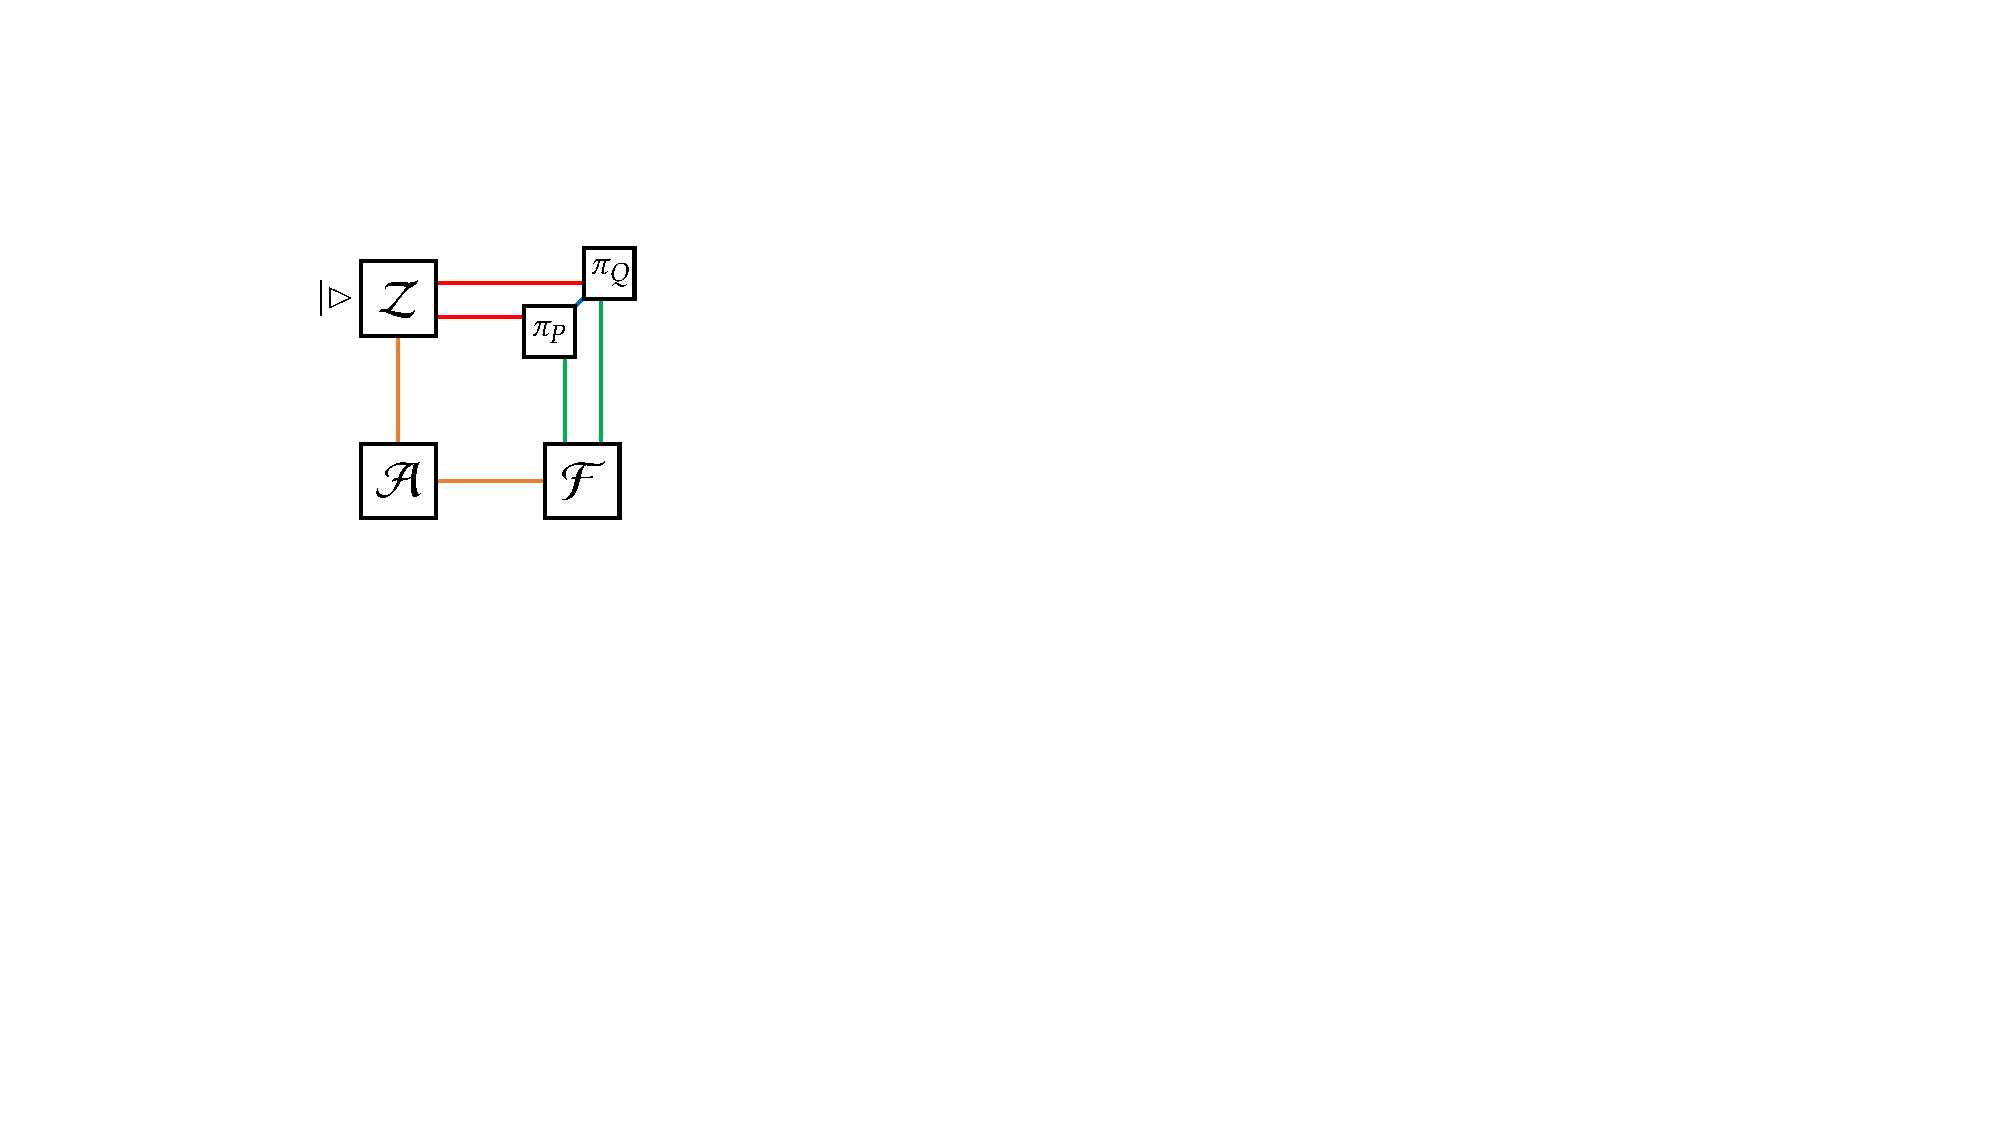
\includegraphics[width=\linewidth]{graphics/execUC-colored}
\end{subfigure}
\caption{Full definition of \textsf{execUC}. The channels follow a uniform
naming scheme. The read end of a channel is prefixed with \textsf{r-} and the
write end of a channel is prefixed with \textsf{w-}. The channel \textsf{rZ2P}
denotes the read end of communications from the environment \textsf{z} to the
party \textsf{p}. First, the random bitstring is split amongst each of the five
parties. Then, the functionality, the adversary, and both protocol parties are
spawned in a child process (given the appropriate channels and parameters), and
the process continues as the environment process. Notice that parties are run in
wrapper functions, which alter their behavior depending on whether or not they
are corrupted. If a party is corrupted, then the adversary masquerades as the
party. The mode carried over the rightmost lollipop is derived as $\{(\mathsf{m}_{\mathsf{f}},\mathsf{m}_{\mathsf{a}},\mathsf{m_{\mathsf{z}}) \mid \mathsf{m}_{\mathsf{f}}
|| (\mathsf{m}_{\mathsf{a}} || (\mathsf{R} || (\mathsf{R}
|| \mathsf{m}_{\mathsf{z}}))) => \mathsf{m}}\}$.}
\label{fig:execUC}
\end{figure*}
\newpage
\twocolumn

\section{Extending ILC with Trapdoor Permutations}

UC Commitments are realized from cryptographic primitives, such as trapdoor
permutations, which require extensions to ILC. The new syntactic forms are
\textsf{kgen}, \textsf{tdp}, \textsf{inv}, and \textsf{hc} with the static and
dynamic semantics shown in Figure~\ref{fig:extended-ilc}. The semantics are
written in terms of the cryptographic objects themselves.

The key generation function \textsf{keygen} takes as input a random bitstring
and outputs a random public key $v_{pk}$ and a trapdoor $v_{td}$. The trapdoor
permutation function
\textsf{tdp} takes as inputs a key $v_{pk}$ and a bitstring $v_{in}$ and outputs
a bitstring $v_{out}$. The \textsf{inv} function takes as inputs a key-trapdoor
pair $(v_{pk}, v_{td})$ and a bitstring $v_{in}$ and outputs a bitstring
$v_{out}$. The hardcore predicate function
\textsf{hc} takes as input a key $v_{pk}$ and outputs a single bit.

\begin{figure*}
  \begin{grammar}
    Expressions
    & $e$
        &$\bnfas$&
        $\eKGen{e} \bnfalt \eTdp{e_1}{e_2} \bnfalt \eHc{e}$
  \end{grammar}
  
  \judgbox{\Delta ; \Gamma |- e : A |> m}{~~Under $\Delta$ and $\Gamma$, expression~$e$ has
  intuitionistic type $A$ and mode $m$.}
  \begin{mathpar}
  \Infer{kgen}
  {\Delta ; \Gamma |- e : [\tyBit]}
  {\Delta; \Gamma |- \eKGen{e}: [\tyBit]}
  %
  \and
  %
  \Infer{eTdp}
  {\Delta_1; \Gamma |- e_1 : [\tyBit]\\
   \Delta_2; \Gamma |- e_2 : [\tyBit]}
  {\Delta_1, \Delta_2; \Gamma |- \eTdp{e_1}{e_2}: [\tyBit]}
  %
  \and
  %
  \Infer{hc}
  {\Delta; \Gamma |- e : \tyArr{[\tyBit]}{}{\tyArr{[\tyBit]}{}{[\tyBit]}}}
  {\Delta; \Gamma |- \eHc{e}: \tyBit}
  \end{mathpar}
  
  \judgbox{\Store_1 ; e_1 ---> \Store_2 ; e_2}{~~Under store $\Store_1$,
    expression~$e_1$ reduces to~$\Store_2 ; e_2$.}
  \begin{mathpar}
  \Infer{kgen}
  {\keyword{\textbf{Gen}}(n) = (v_{pk}, v_{td}) \\ v_{pk}, v_{td} \in \{0,1\}^n}
  { \Store ; \eKGen{n} ---> \Store ; (v_{pk}, v_{td})}
  \and
  \Infer{tdp}
  {\mathbf{f}_{v_k}(v_i) = v_o \\ \mathbf{f} \colon \{0,1\}^n -> \{0,1\}^n -> \{0,1\}^n}
  { \Store ; \eTdp{v_k}{v_i} ---> \Store ; v_o }
  \and
  \Infer{hc}
  {\keyword{\textbf{Hc}}(\mathbf{f}_{v_k}) = v \\ \keyword{\textbf{Hc}} \colon
  (\{0,1\}^n -> \{0,1\}^n) -> \{0, 1\}}
  { \Store ; \eHc{f_{v_k}} ---> \Store ; v}
  \end{mathpar}
%  \begin{mathpar}
%    G_{pk}(r) = (f^{(3n)}_{pk}(r), B(f^{(3n-1)}_{pk}(r)), \ldots, B(f_{pk}(r)), B(r))
%  \end{mathpar}
  \caption{ILC extended with trapdoor permutations.}
  \label{fig:extended-ilc}
\end{figure*}


We can use these to implement a special pseudorandom number generator $G_{pk}
\colon \{0,1\}^k \to \{0,1\}^{4k}$ that has a trapdoor property, i.e., it is easy
to compute, but difficult to invert except with special information called the
``trapdoor.''
\[ G_{pk}(r) = \big(\mathbf{f}_{pk}^{(3n)}(r),
\mathbf{B}(\mathbf{f}_{pk}^{(3n-1)}(r)), \ldots, \mathbf{B}(\mathbf{f}_{pk}(r)),
\mathbf{B}(r)\big)\]
\noindent Here, $\mathbf{f}_{pk}$ is a trapdoor permutation over $\{0,1\}^{k}$,
with $\mathbf{f}_{pk}^{(i)}(r)$ denoting the $i^{\textnormal{th}}$-fold
application of $\mathbf{f}_{pk}$, and $\mathbf{B}$ is a hardcore predicate for
$\mathbf{f}_{pk}$. In ILC, this can be implemented as:
\lstinputlisting[style=myilc]{listings/prg.ilc}

\section{Universally Composable Commitment Protocol}
\label{app:ucc}
In this section we give the full elaboration of our UC commitment instantiation.
The specification functionality is given in the body in Figure~\ref{func:com},
along with the protocol implementation in Section~\ref{subsec:example}.
Our development follows closely from the psuedocode in the UC literature~\cite{canetti2001commitments}, which we show here in Algorithm~\ref{alg:com}.
The protocol relies on the CRS functionality which we define here in Figure~\ref{fig:f-crs}.
To briefly summarize what is going: the setup CRS samples a random string $\sigma$ and two trapdoor pseudorandom generators (prgs $\mathsf{pk}_0, \mathsf{pk}_1$).
To commit to the bit $b$, the commiter produces a string $y$ that is the result of applying one or the other of the prgs, and if $b=1$ additionally applying xor with $\sigma$.
The intuitive explanation why this is hiding is that without the trapdoor, it is difficult to tell whether a random $4k$-bit string is in the range of either prg. To open the commitment, the committer simply reveals the preimage and the receiver checks which of the two cases applies. The intuitive explanation why this is binding is that it is difficult to find a pair $y,y\oplus\sigma$ that are respectively in the range of both prgs.

The UC proof consists of two simulators, one for the ideal world and one for the real world.
The ideal world simulator, given in Figure~\ref{fig:sim} is ported directly from the UC literature~\cite{canetti2001commitments}, while the non-standard real world simulator, given in Figure~\ref{fig:simR}, is required because our protocol emulation definition requires simulation in both directions.
The key to the ideal world simulator is to allow the simulator to generate its own ``fake'' CRS, for which it stores the trapdoors. The string $\sigma$ is not truly random, but instead is the result of combining two evaluations of the prgs.
The ideal world simulator consists of two cases, depending on which of the parties is corrupt.

In the case that the committer P is corrupt, the simulator needs to be able to \emph{extract} the committed value. The simulator is activated when $\mc{Z}$ sends a message $(\mathsf{Commit}' ~ y)$; in the real world, this is relayed by the dummy adversary to Q, who outputs \textsf{Committed} back to the environment. Hence to achieve the same effect in the ideal word, the simulator must send $(\mathsf{Commit}~b)$ to $\Func_{\textsc{Com}}$. To extract $b$ from $y$, the simulator makes use of the prg trapdoor check which one has $y$ in its range.
It is necessary to argue by cryptographic reduction that this simulation is sound.
To show this, we would define an alternative execution where the prg is substituted for a truly random function (i.e., a random oracle). If an environment $\mc{Z}$ could distinguish between these two worlds, then we could adapt the execution to distinguish the prg from random, violating the prg assumption.

In the case that the receiver Q is corrupt, the simulator needs to \emph{equivocate}.
The simulator is activated when $\mc{Z}$ inputs $(\mathsf{Commit}~b)$ to P, after which $\Func_{\textsc{Com}}$ sends $\mathsf{Committed}$ to the simulator.
In the real world, the environment receives a commitment message $(\mathsf{Commit}'~y)$ from corrupted Q for some seemingly-random $y$. To achieve the same effect, the simulator must choose $y$. However, the simulator is next activated when the $\mc{Z}$ inputs $(\mathsf{Open}~b)$ to P, after which the simulator learns $b$ from $\Func_{\textsc{Com}}$. However, in the real world the environment receives a valid opening $(\mathsf{Opened}'~b~r)$ that is consistent with  $y$ and with the value chosen by the environment. Thus the simulator must initially choose $y$ so that it can later be opened to either value $b$ may take. The simulator achieves this by choosing $\sigma$ and $y$ ahead of time while generating the fake CRS. The reduction step is the same, and involves replacing prg with a true random function.

Recall that the motivation for the real world simulator is to rule out degenerate protocols that diverge in some way.
For every well behaved environment such that the ideal world is \textsf{PPT}, we need to demonstrate an adversary in the real world that is also \textsf{PPT}.
Fortunately, the real world simulator, shown in Figure~\ref{fig:simR} is much simpler than ideal world simulator.
Essentially the simulator runs a copy of the honest protocol for each of the corrupted parties. The simulation that results in this case is identical.

\begin{algorithm}
\SetAlgorithmName{Protocol}{protocol}{List of Protocols}
\DontPrintSemicolon

\SetKwBlock{Parameters}{\textnormal{\textsf{Public strings}:}}{}
\Parameters{
  $\sigma$: Random string in $\{0,1\}^{4n}$\;
  ${pk}_0, {pk}_1$: Keys for generator $G_{k} \colon \{0,1\}^n \to \{0,1\}^{4n}$
}\smallskip
\SetKwBlock{Commit}{\textnormal{\textsf{Commit}($b$):}}{}
\Commit{
  $r \leftarrow \{0, 1\}^n$\;
  $y \coloneqq G_{{pk}_b}(r)$\;
  if $b=1$ then $y \coloneqq y \oplus \sigma$\;
  Send $(\mathsf{Commit}, y)$ to receiver.\;
  Upon receiving $(\mathsf{Commit}, y)$ from $A$, $B$ outputs $(\mathsf{Receipt})$.
}\smallskip

\SetKwBlock{Decommit}{\textnormal{\textsf{Decommit}($x$):}}{}
\Decommit{
  Send $(b, r)$ to receiver.\;
  Receiver checks $y = G_{{pk}_b}(r)$ for $b = 0$, or $y = G_{{pk}_b}(r) \oplus \sigma$
  for $b = 1$. If verification succeeds, then $B$ outputs $(\mathsf{Open}, b)$.
}
\caption{Universally Composable Commitment}
\label{alg:com}
\end{algorithm}

\begin{figure*}
\lstinputlisting[style=myilc]{listings/dummy.ilc}
\caption{Dummy adversary. The dummy adversary forwards messages from the
environment to either the functionality (if the message has
constructor \textsf{A2F}) or the party \textsf{p} (if the message has
constructor \textsf{A2P}). Similarly, the dummy adversary forwards messages from
the functionality or the procotol parties to the environment.}
\label{fig:dummy-adversary}
\end{figure*}

\begin{figure*}
\lstinputlisting[style=myilc]{listings/dummyp.ilc}
\caption{Dummy party. The dummy party simply relays information between the
environment and the functionality.}
\label{fig:dummy-party}
\end{figure*}

\begin{figure*}
\lstinputlisting[style=myilc]{listings/Fcrs.ilc}
\caption{Ideal functionality for common reference string.}
\label{fig:f-crs}
\end{figure*}

\begin{figure*}
\lstinputlisting[style=myilc]{listings/Fcom-full.ilc}
\caption{Ideal functionality for one-time bit commitment.}
\label{fig:f-com-full}
\end{figure*}

\begin{figure}
\lstinputlisting[style=myilc]{listings/sim.ilc}
\caption{Ideal world simulator for UC commitment.}
\label{fig:sim}
\end{figure}

\begin{figure*}
\lstinputlisting[style=myilc]{listings/simR.ilc}
\caption{Real world simulator for UC commitment.}
\label{fig:simR}
\end{figure*}
